\subsection{Applicability of Model to Real Data}
Now that we have parameterized patient function curves, we can explore the relationship between various covariates and curve parameters.  Recall from previous plots that the covariates that seem to affect the curve shape the most are age and the pre-treatment function level.  On the following few pages, for each of the 3 side effect function values, and for each of treatments, and for each of those 2 covariates, we make 4 scatter plots.  For each scatter plot, the x-axis is the covariate, and the y-axis is 1 of 4 curve parameters: $a, b, c$, and also the quantity $a+(1-a)b$, which is equal to the total initial drop in function value, relative to the pre-treatment function value.  This last quantity is labelled as 'drop' in the scatter plots.  Trends in these scatter plots would lead us to believe that the coefficients in the generalized linear models for the $a, b, c$ parameters would be non-zero.

\begin{figure}
\centering
\begin{subfigure}{
  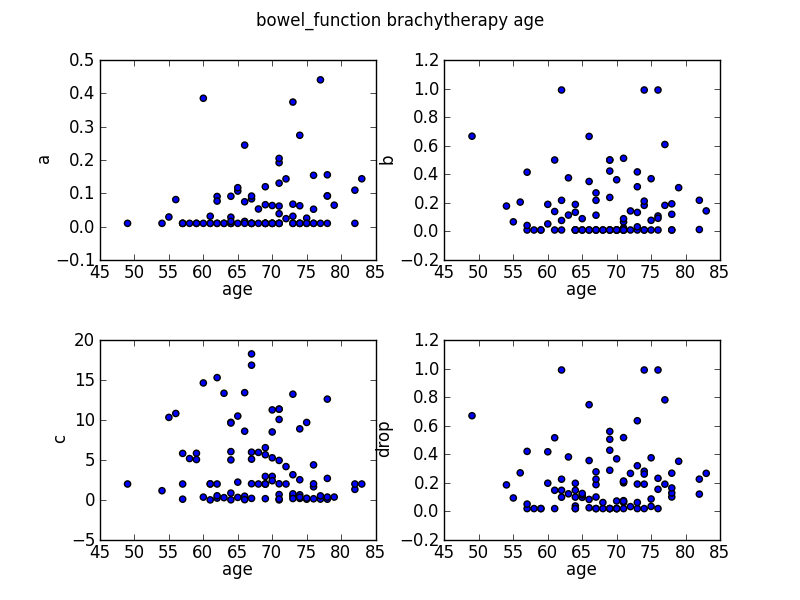
\includegraphics[width=.45\linewidth,height=0.3\textheight]{/Users/glareprotector/prostate_git/glare/tex_files/sections/exploratory_with_abc/files/attribute_vs_curve_parameters/bowel_function_brachytherapy_age.png}}
\end{subfigure}
\begin{subfigure}{
  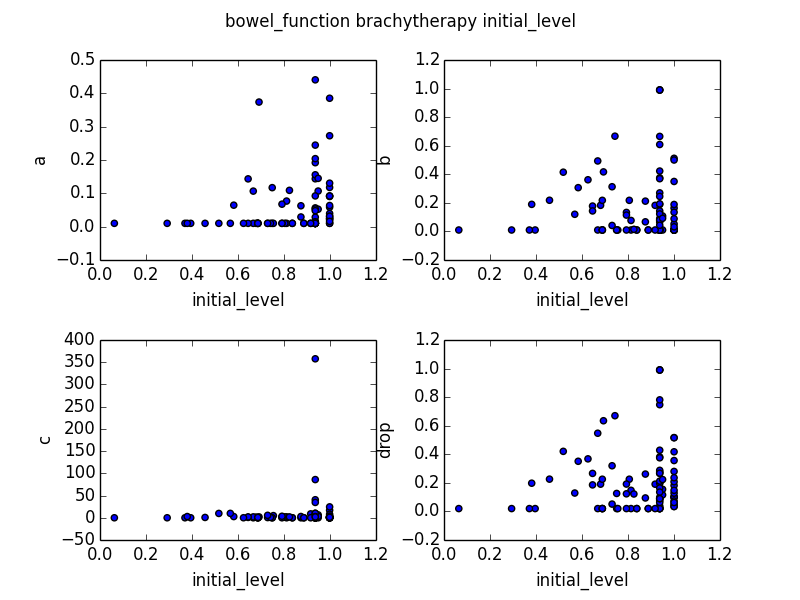
\includegraphics[width=.45\linewidth,height=0.3\textheight]{/Users/glareprotector/prostate_git/glare/tex_files/sections/exploratory_with_abc/files/attribute_vs_curve_parameters/bowel_function_brachytherapy_initial_level.png}}
\end{subfigure}
\begin{subfigure}{
  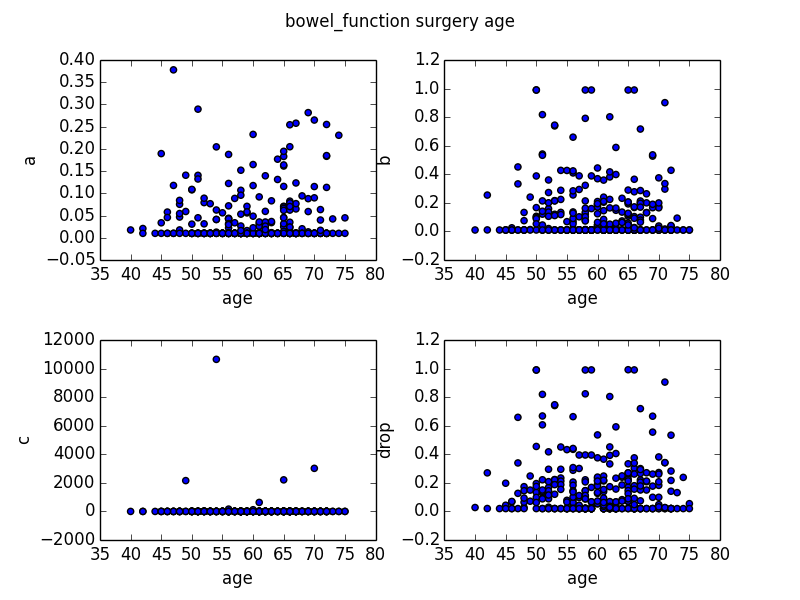
\includegraphics[width=.45\linewidth,height=0.3\textheight]{/Users/glareprotector/prostate_git/glare/tex_files/sections/exploratory_with_abc/files/attribute_vs_curve_parameters/bowel_function_surgery_age.png}}
\end{subfigure}
\begin{subfigure}{
  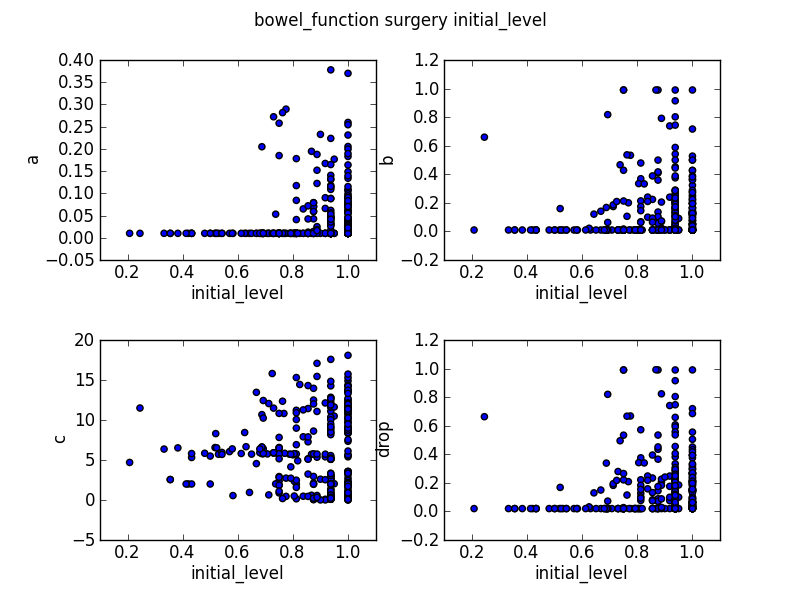
\includegraphics[width=.45\linewidth,height=0.3\textheight]{/Users/glareprotector/prostate_git/glare/tex_files/sections/exploratory_with_abc/files/attribute_vs_curve_parameters/bowel_function_surgery_initial_level.png}}
\end{subfigure}
\begin{subfigure}{
  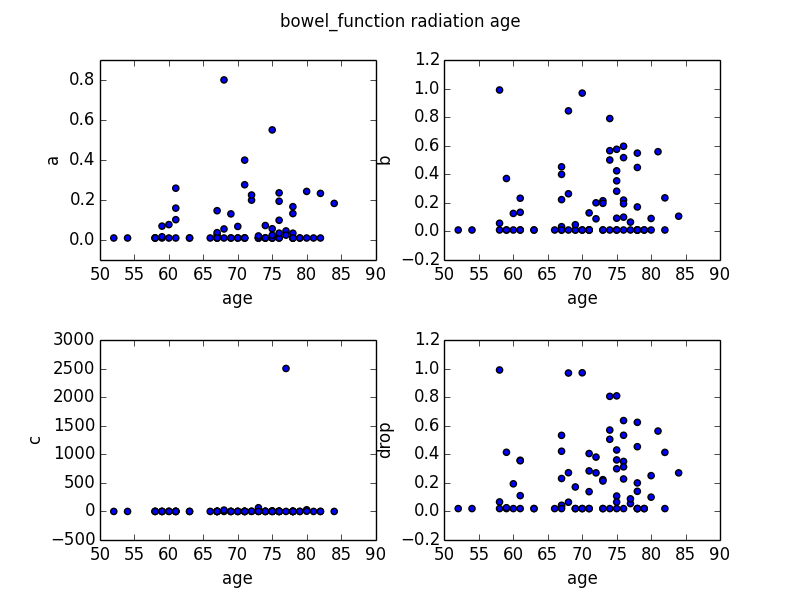
\includegraphics[width=.45\linewidth,height=0.3\textheight]{/Users/glareprotector/prostate_git/glare/tex_files/sections/exploratory_with_abc/files/attribute_vs_curve_parameters/bowel_function_radiation_age.png}}
\end{subfigure}
\begin{subfigure}{
  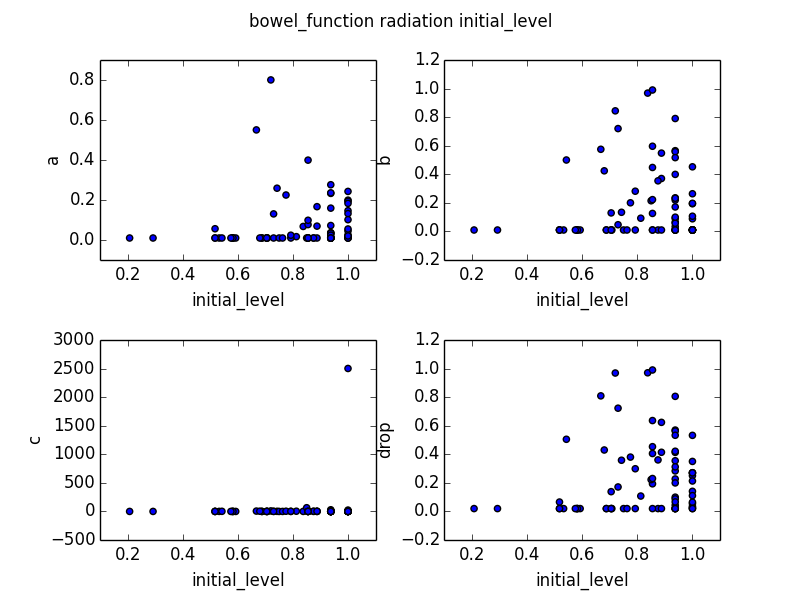
\includegraphics[width=.45\linewidth,height=0.3\textheight]{/Users/glareprotector/prostate_git/glare/tex_files/sections/exploratory_with_abc/files/attribute_vs_curve_parameters/bowel_function_radiation_initial_level.png}}
\end{subfigure}
\caption{Plots of bowel function curve parameters vs initial function level and age attribute, stratified by treatment}
\end{figure}

\begin{figure}
\centering
\begin{subfigure}{
  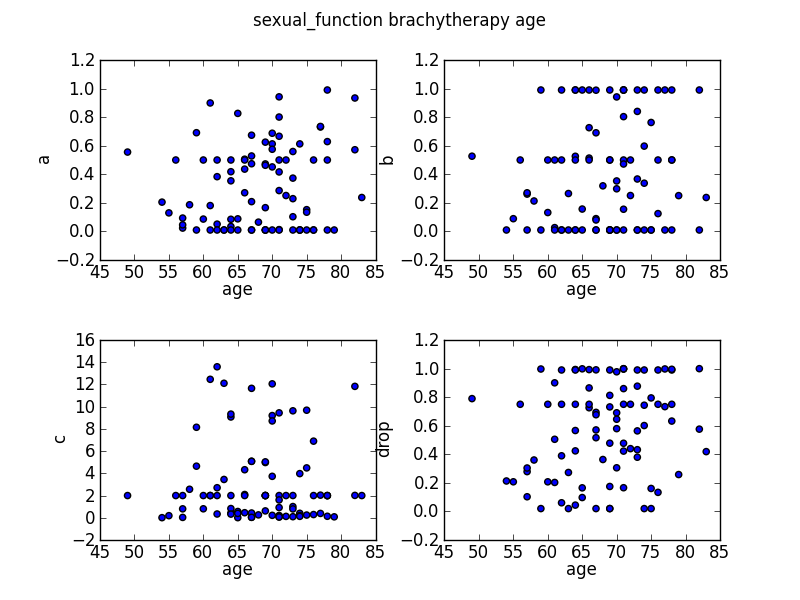
\includegraphics[width=.45\linewidth,height=0.3\textheight]{/Users/glareprotector/prostate_git/glare/tex_files/sections/exploratory_with_abc/files/attribute_vs_curve_parameters/sexual_function_brachytherapy_age.png}}
\end{subfigure}
\begin{subfigure}{
  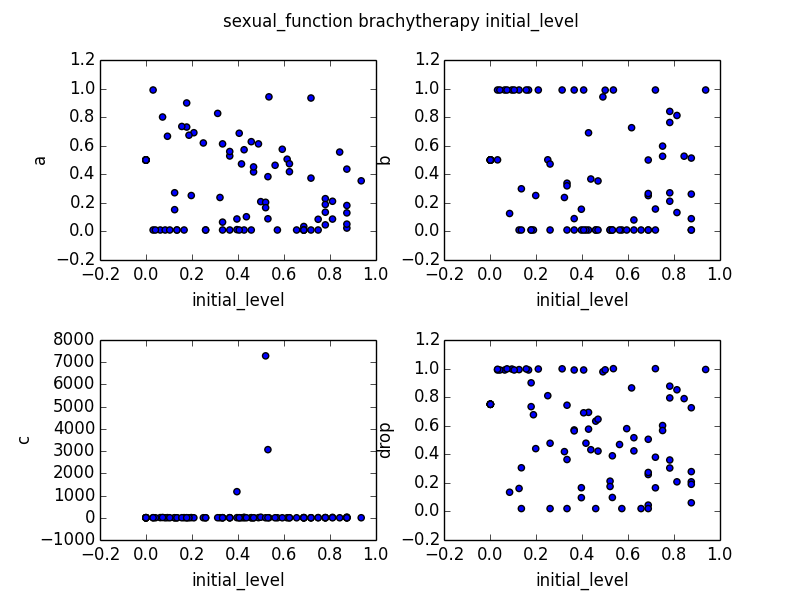
\includegraphics[width=.45\linewidth,height=0.3\textheight]{/Users/glareprotector/prostate_git/glare/tex_files/sections/exploratory_with_abc/files/attribute_vs_curve_parameters/sexual_function_brachytherapy_initial_level.png}}
\end{subfigure}
\begin{subfigure}{
  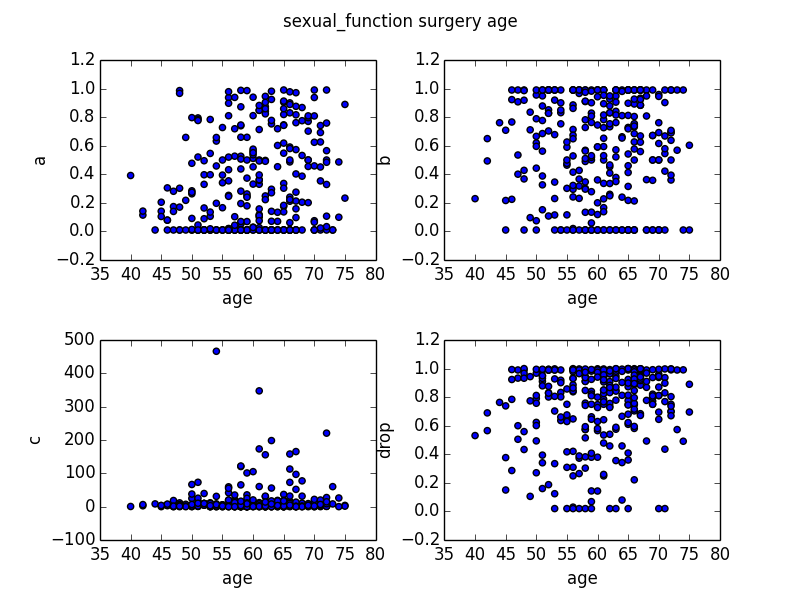
\includegraphics[width=.45\linewidth,height=0.3\textheight]{/Users/glareprotector/prostate_git/glare/tex_files/sections/exploratory_with_abc/files/attribute_vs_curve_parameters/sexual_function_surgery_age.png}}
\end{subfigure}
\begin{subfigure}{
  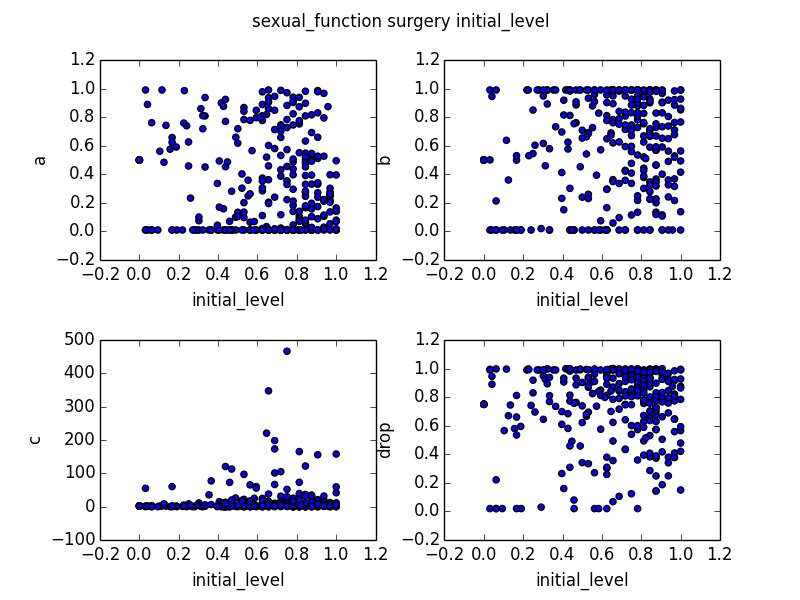
\includegraphics[width=.45\linewidth,height=0.3\textheight]{/Users/glareprotector/prostate_git/glare/tex_files/sections/exploratory_with_abc/files/attribute_vs_curve_parameters/sexual_function_surgery_initial_level.png}}
\end{subfigure}
\begin{subfigure}{
  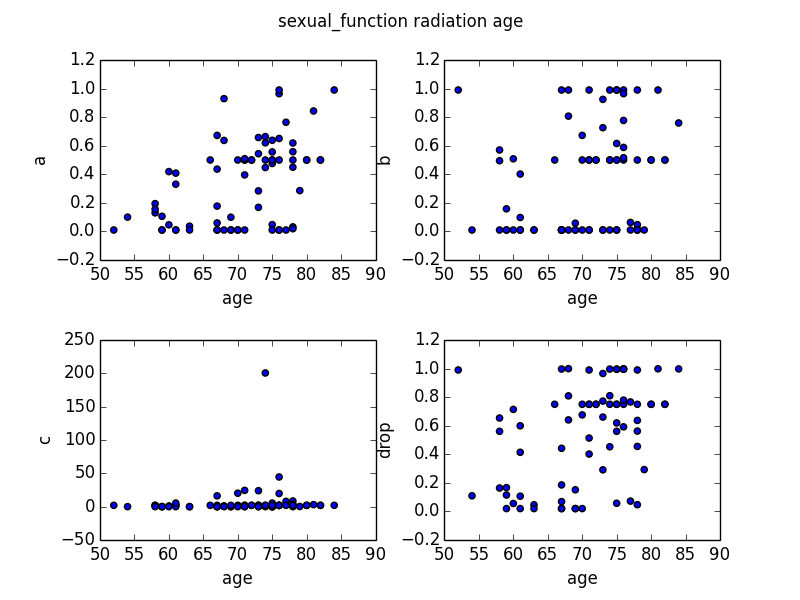
\includegraphics[width=.45\linewidth,height=0.3\textheight]{/Users/glareprotector/prostate_git/glare/tex_files/sections/exploratory_with_abc/files/attribute_vs_curve_parameters/sexual_function_radiation_age.png}}
\end{subfigure}
\begin{subfigure}{
  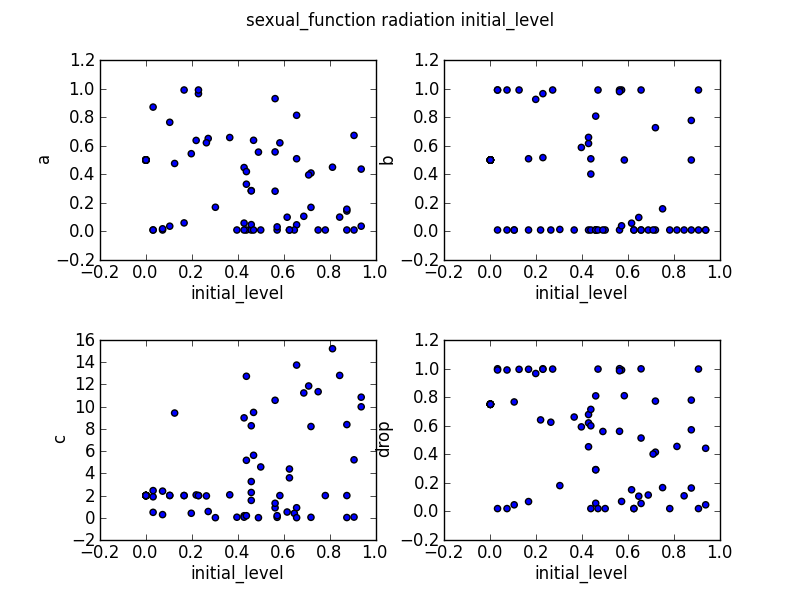
\includegraphics[width=.45\linewidth,height=0.3\textheight]{/Users/glareprotector/prostate_git/glare/tex_files/sections/exploratory_with_abc/files/attribute_vs_curve_parameters/sexual_function_radiation_initial_level.png}}
\end{subfigure}
\caption{Plots of sexual function curve parameters vs initial function level and age attribute, stratified by treatment}
\end{figure}

\begin{figure}
\centering
\begin{subfigure}{
  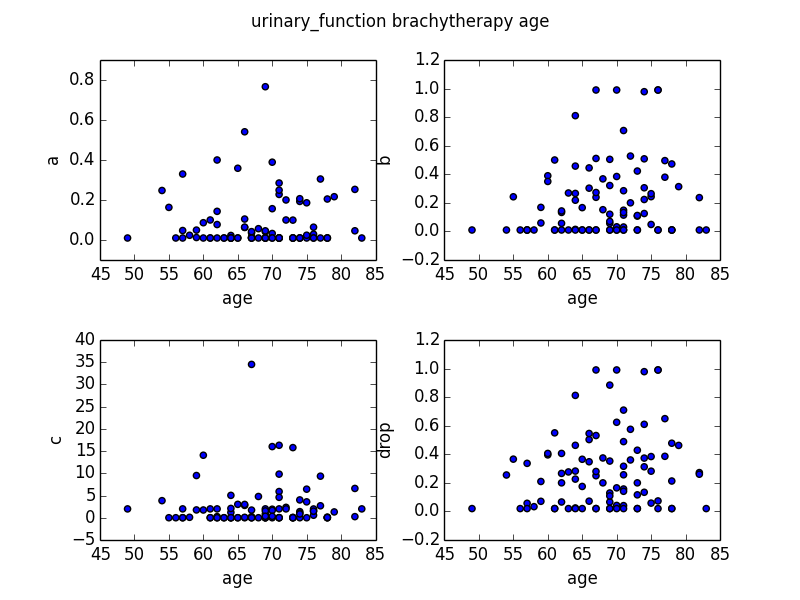
\includegraphics[width=.45\linewidth,height=0.3\textheight]{/Users/glareprotector/prostate_git/glare/tex_files/sections/exploratory_with_abc/files/attribute_vs_curve_parameters/urinary_function_brachytherapy_age.png}}
\end{subfigure}
\begin{subfigure}{
  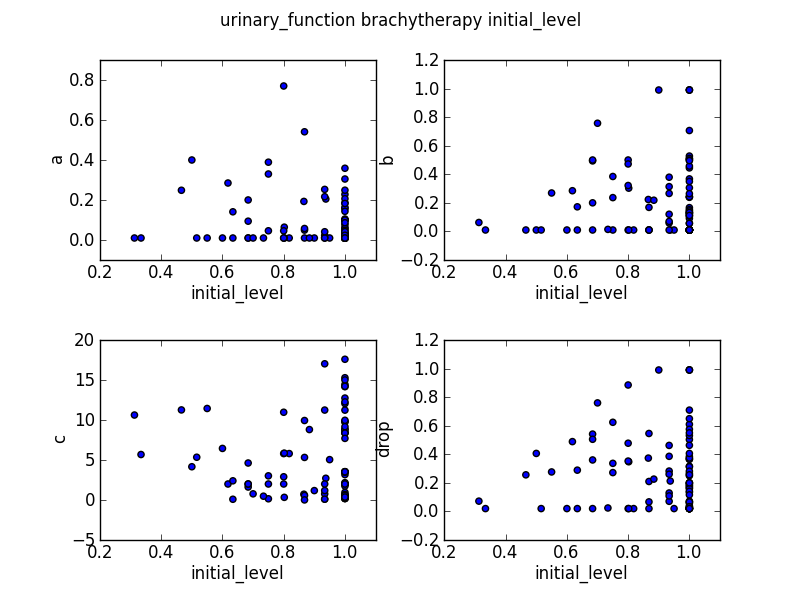
\includegraphics[width=.45\linewidth,height=0.3\textheight]{/Users/glareprotector/prostate_git/glare/tex_files/sections/exploratory_with_abc/files/attribute_vs_curve_parameters/urinary_function_brachytherapy_initial_level.png}}
\end{subfigure}
\begin{subfigure}{
  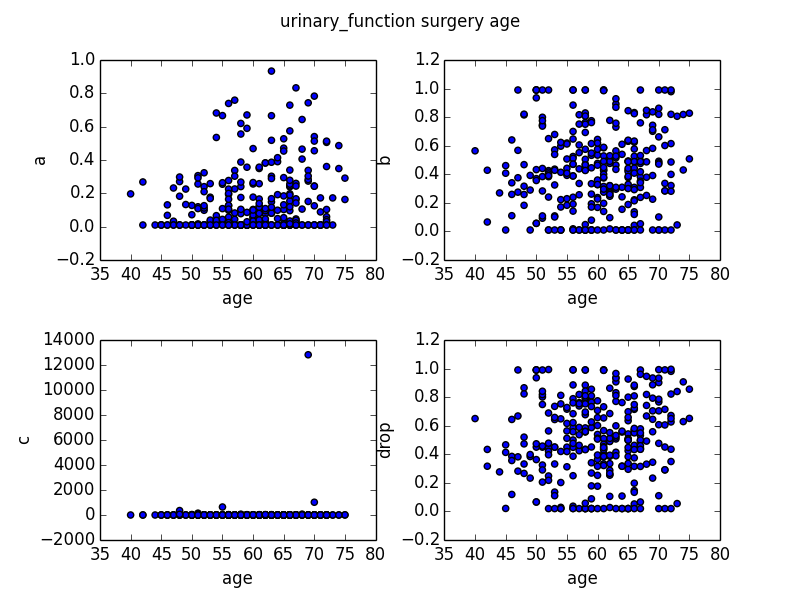
\includegraphics[width=.45\linewidth,height=0.3\textheight]{/Users/glareprotector/prostate_git/glare/tex_files/sections/exploratory_with_abc/files/attribute_vs_curve_parameters/urinary_function_surgery_age.png}}
\end{subfigure}
\begin{subfigure}{
  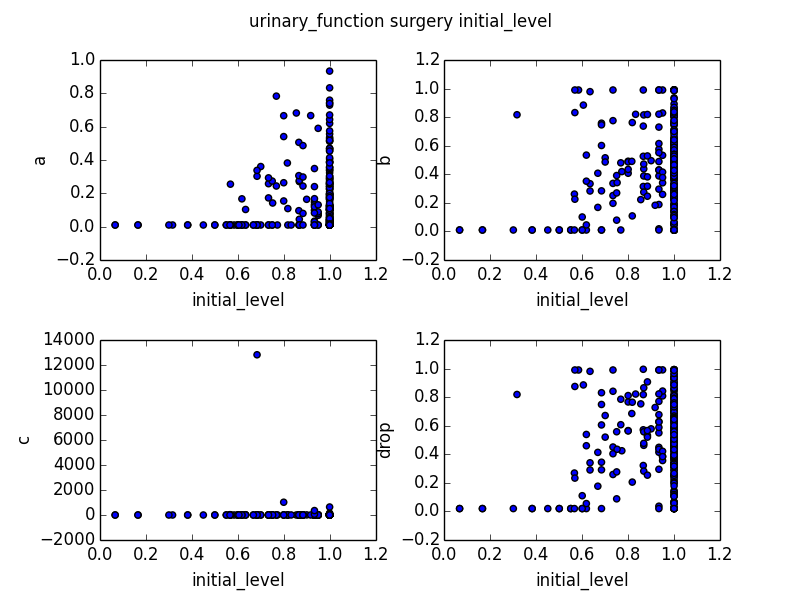
\includegraphics[width=.45\linewidth,height=0.3\textheight]{/Users/glareprotector/prostate_git/glare/tex_files/sections/exploratory_with_abc/files/attribute_vs_curve_parameters/urinary_function_surgery_initial_level.png}}
\end{subfigure}
\begin{subfigure}{
  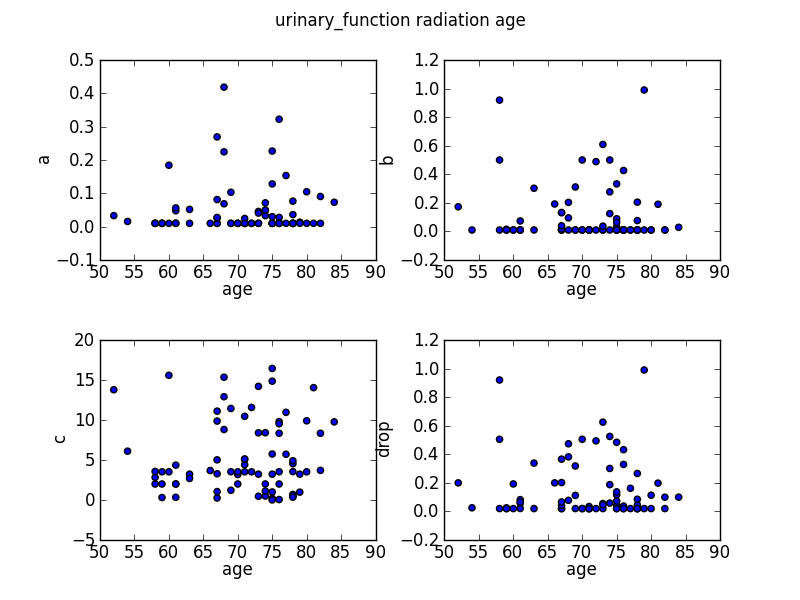
\includegraphics[width=.45\linewidth,height=0.3\textheight]{/Users/glareprotector/prostate_git/glare/tex_files/sections/exploratory_with_abc/files/attribute_vs_curve_parameters/urinary_function_radiation_age.png}}
\end{subfigure}
\begin{subfigure}{
  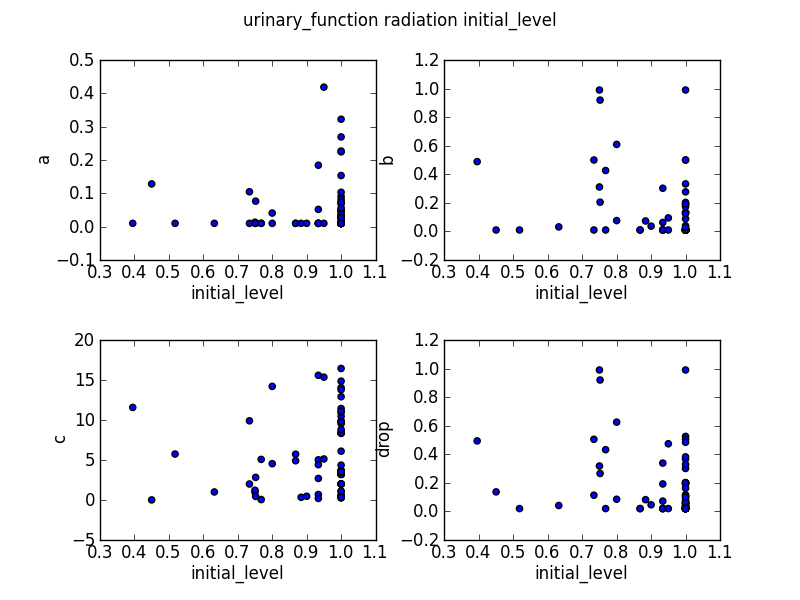
\includegraphics[width=.45\linewidth,height=0.3\textheight]{/Users/glareprotector/prostate_git/glare/tex_files/sections/exploratory_with_abc/files/attribute_vs_curve_parameters/urinary_function_radiation_initial_level.png}}
\end{subfigure}
\caption{Plots of sexual function curve parameters vs initial function level and age attribute, stratified by treatment}
\end{figure}